\documentclass[a4paper, 11pt]{article}
\usepackage{comment} % enables the use of multi-line comments (\ifx \fi) 
\usepackage{fullpage} % changes the margin
\usepackage[swedish]{babel}
\usepackage{enumitem}
\usepackage{graphicx}
\graphicspath{ {images/} }
\usepackage[utf8]{inputenc}


\begin{document}
\begin{center}
\LARGE \bf 14.02 Principles of Macroeconomics\\ Problem Set 1
\end{center}

\vspace{1cm} 
\noindent\textbf{Name: }Faaya Abate Fulas \\

\section*{Question 1: Economic Data}
\begin{enumerate}[label=\textbf{(\alph*)}]
\item \textbf{Unemployment and Non-employment}
\begin{enumerate}[label=\textbf{\arabic*.}]
\item 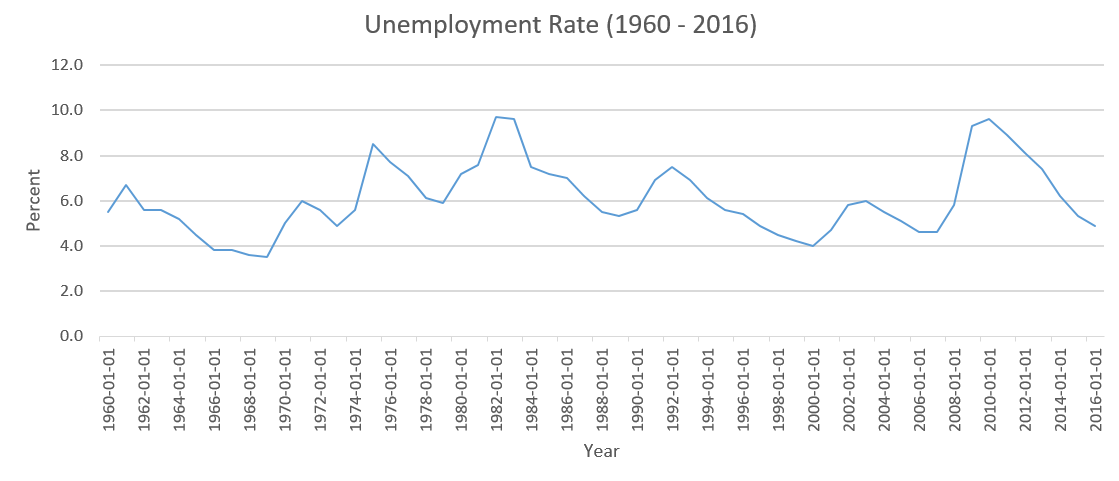
\includegraphics[scale=0.7]{unemployment_rate}
\item 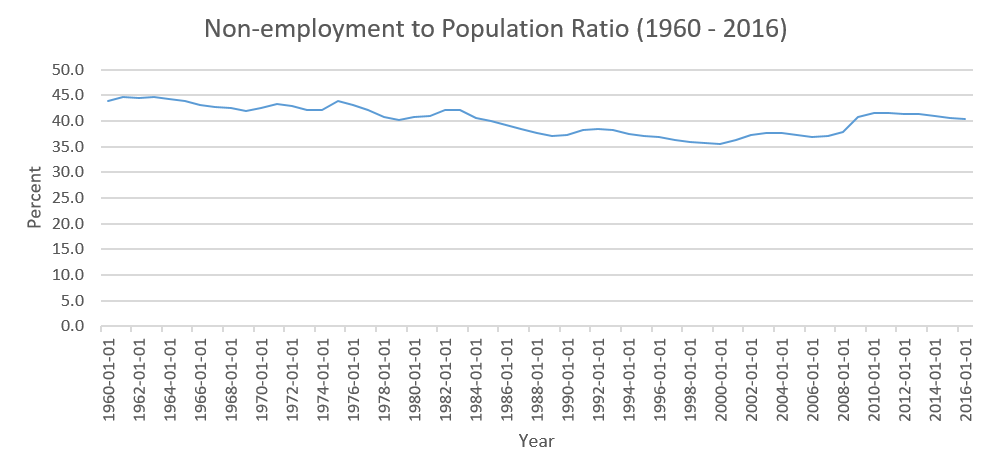
\includegraphics[scale=0.8]{non-employment}
\item The unemployment rate is the ratio of the number of unemployed people in the labor force to the number of people in the labor force, where as non-employment-to-population ratio is the ratio of the number of people without a job, including those that are not in the labor force, to the entire population. \\

No. The unemployment rate was $4.6\%$ in 2006 and $4.9\%$ in 2016. \\

No. The non-employment-to-population ratio was $36.9\%$ in 2006 and $40.3\%$ in 2016. \\

\end{enumerate}
\clearpage
\item \textbf{Okun's Law and Phillips Curve}

\begin{enumerate}[label=\textbf{\arabic*.}]
\setcounter{enumi}{4}
\item 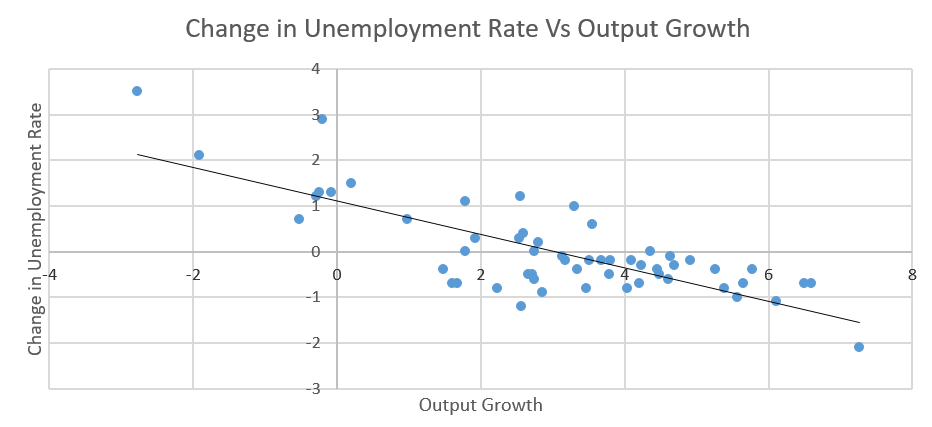
\includegraphics[scale = 0.83]{okuns_law}
\item 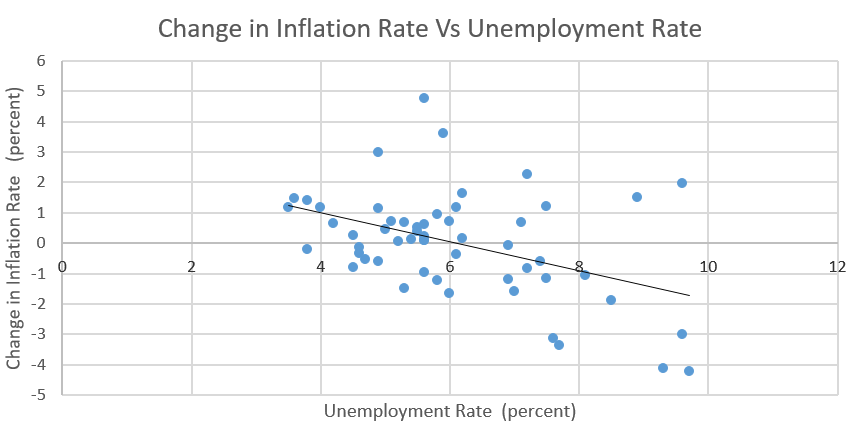
\includegraphics[scale = 0.9]{philips_curve}
\end{enumerate}
\end{enumerate}


\section*{Question 2: NGDP, RGDP, Inflation}
\begin{enumerate}[label=\textbf{(\alph*)}]
\item \textbf{Three Ways to Measure GDP}
\begin{enumerate}[label=\textbf{\arabic*.}]
\item Steel and Oil are intermediate goods since they are used to manufacture other goods in the market. Cars are the only final good in the economy, so the GDP is equal to the revenue from the sales of cars, \$500
\item Value added by a firm = Value of its production - Value of intermediate goods used in its production\\

Steel Company: \$130 - \$40 = \$90\\
Oil Company: \$200 - \$110 = \$90\\
Car Company: \$500 - \$180 = \$320\\

Therefore, GDP= \$90 + \$90 + \$320 = \$500
\clearpage
\item For each firm in the economy, Total Income = Labor Income + Profit Income\\

Steel Company: \$10 + \$80 = \$90\\
Oil Company: \$70 + \$20 = \$90\\
Car Company: \$220 + \$100 = \$320\\

Therefore, GDP= \$90 + \$90 + \$320 = \$500


\end{enumerate}
\item \textbf{Real and Nominal GDP}

\begin{center}
 \begin{tabular}{||c| c| c| c ||} 
 \hline
 $Year$ & $NGDP$ & $RGDP_{2015}$ & $GDP$ $Deflator (P_t)$\\ [0.5ex] 
 \hline
 \hline
 2014 & 5*2000 + 10*200 = \$12,000 & 5*1000 + 10*400 = \$9,000& $\frac{12000}{9000} = 1.33$ \\ 
 \hline
 2015 & 10*1000 + 20*400 = \$18,000 & \$18,000& 1\\
 \hline
 2016 & 12*1200 + 30*200 = \$20,400 & 12*1000 + 30*400 = \$24,000&$\frac{20400}{24000} = 0.85$ \\ [1ex] 
 \hline
\end{tabular}
\end{center}


 Inflation Rate between year 2014 and 2015: \\
 $\pi_{2015} = \frac{(P_{2015} - P_{2014})}{P_{2014}} = 0.03/1.33= 0.25$\\
 
 Inflation Rate between year 2015 and 2016: \\
 $\pi_{2016} = \frac{(P_{2016} - P_{2015})}{P_{2015}} = -0.15$
\end{enumerate}
\section*{\textbf{Question 3: Government Spending Multiplier}}
\begin{enumerate}[label=\textbf{(\alph*)}]
\item \textbf{Exogenous G and T}
\begin{enumerate}[label=\textbf{\arabic*.}]
\item $ Y = Z$,  $Z = C + I + G$ and $C = c_0 + c_1(Y - T)$\\

$Y = c_0 + c_1Y-c_1T + I +G$\\
$(1-c_1)Y = c_0 + I +G - c_1T$\\
$Y = \frac{1}{1-c_1} (c_0 + I + G - c_1T)$\\

\item Government spending multiplier: $\frac{\partial Y}{\partial G} = \frac{1}{1-c_1}$\\

The increase in output is larger than the initial shift in demand because an increase in government spending(G) increases demand(Z). The increase in demand leads to an increase in production which then leads to an increase in income(Y). So, the effect is an increasing geometric convergence towards the point of equilibrium.  

\item $S = Y - T - C$ and $Y = C + I + G$\\

$S = C + I + G - T -C$\\
$S = I + G - T$\\
$I = S + (T - G)$\\

\item $\frac{\partial S}{\partial G} = 1$

\end{enumerate}
\clearpage
\item \textbf{Balanced Budget, G = T}
\begin{enumerate}[label=\textbf{\arabic*.}]
\item $Y = \frac{1}{1-c_1} (c_0 + I + G - c_1T)$ and $T = G$\\

$Y = \frac{1}{1-c_1} (c_0 + I + G - c_1G)$\\
$Y = \frac{1}{1-c_1} (c_0 + I +(1-c_1)G)$\\

\item  Government spending multiplier: $\frac{\partial Y}{\partial G} = 1$\\

Since $0<c_1<1$, $\frac{1}{1-c_1} > 1$. The balanced budget multiplier indicates  that the impact of an increase in government spending (G) in one cycle is matched by a proportional increase in taxes (T) on the next cycle. All subsequent increases in T and G offset each other, so the overall impact on aggregate production will just be the initial shift. \\

\item $S = S + (T-G)$ and $T=G$\\

$ I = S $\\
\item Private saving is not affected by government saving
\end{enumerate}
\item \textbf{Endogenous Tax Revenue}
\begin{enumerate}[label=\textbf{\arabic*.}]
\item $Y = c_0 + c_1Y-c_1T + I +G$ and $T= t_0 + t_1Y$\\

$Y = c_0 + c_1Y-c_1t_0 - c_1t_1Y + I +G$\\
$(1-c_1+c_1t_1)Y = c_0 -c_1t_0+ I +G$\\
$Y = \frac{1}{1-c_1+c_1t_1} (c_0 - c_1t_0 + I + G )$\\
\item  Government spending multiplier: $\frac{\partial Y}{\partial G} = \frac{1}{1-c_1+c_1t_1}$\\

Since $ 0 < c_1 < 1$ and $0 < t_1 < 1$, $c_1t_1 < c_1$. Therefore, $1< \frac{1}{1-c_1+c_1t_1} <\frac{1}{1-c_1}$. \\ 

This multiplier indicates that the initial shift in G introduces an increase in income(Y) on the next cycle. The increase in Y, in turn, leads to an increase in taxes(T) since T is an increasing function of Y. The increase in taxes, introduces a subsequent decrease in income. So, instead of a uniform geometric convergence to the equilibrium point as in \textbf{part (a) }where both T and G were exogenous variables, T's dependence on Y leads to an oscillatory geometric convergence to a lower equilibrium point.
\item $PS = T - G$ , $T= t_0 + t_1Y$ and $Y = \frac{1}{1-c_1+c_1t_1} (c_0 - c_1t_0 + I + G )$\\

$ PS = t_0 + \frac{t_1}{1-c_1+c_1t_1} (c_0 - c_1t_0 + I + G ) - G$\\

$\frac{\partial PS}{\partial G} =\frac{t_1}{1-c_1+c_1t_1} - 1$\\

\item $\frac{\partial Y}{\partial t_0} =\frac{-c_1}{1-c_1+c_1t_1}$
\end{enumerate}
\end{enumerate}
\end{document}
